\chapter{Usando \maggen}
\label{chap:usos}
\minitoc
Para usar \maggen\ debemos invocar la herramienta mediante la linea de comando, es decir, debemos contar con una terminal\footnote{En sistemas \textit{windows} compatible: win+R y luego \texttt{cmd} y en sistemas \textit{unix}: Alt+f2 y luego \texttt{xterm}} para su ejecución. Por cuestiones de simpicidad y flexibilidad de la herramienta, no se considero el desarrollo de un \textit{front-end} para \maggen. Además, debemos tener en cuenta, que el usuario presentara interes en el resultado generado de \maggen y no de una innecesaria interfaz grafica, que entorpeceria su comportamiento combinatorio con otros comandos.
  
\maggen\ puede ser invocado utilizando una serie de parametros que inciden directamente sobre el resultados producido por la herramienta. En el desarrollo de este capitulo trataremos estos temas en detalles y ademas analizaremos el uso del evaluador generado por \maggen.

\section{Uso de \maggen: Parametros y opciones}
La totalidad de parámetros y opciones de \maggen\ son opcionales. La sintaxis de invocación de la herramienta esta dada por:\\
\begin{center}\texttt{maggen [OPTIONS]}\end{center}
Las opciones son las siguientes:
\begin{description}
\item [-f  file] Definir el archivo de entrada de \maggen\ como \texttt{file}. Si omitimos esta opción \maggen espera la entrada por la entrada estándar (cin) hasta leer el caracter EOF (end of file) \footnote{En sistemas unix el caracter EOF puede ser producido con Ctrl+D dentro de una consola de comandos.}.
\item [-i  header] Incluir \texttt{header} en la generación de código. Genera un \texttt{\#include ``header''} del archivo que referencia esa ruta. Dicha linea, \maggen la agrega al archivo generado.
\item [-fo folder] Define \texttt{folder} como el directorio de salida para \maggen. Si omitimos esta opción, \maggen\ usa el folder por defecto ``\textit{./out\_maggen/}''.
\item [-o  name] Define a \texttt{name} como el nombre de la clase y del archivo generado por \maggen. Si omitimos esta opción, \maggen\ usa por defecto el nombre ``\textbf{mag\_eval}''.
\item [-h] Muestra mensaje de ayuda.
\end{description}
A continuación observemos algunos ejemplo de invocación de \maggen.
\begin{itemize}
\item Si invocamos:\\ \texttt{./maggen -h} obtenemos el siguiente mensaje de ayuda:
\begin{center}
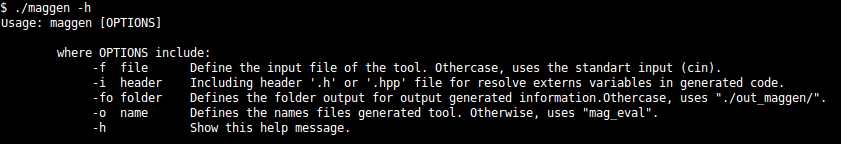
\includegraphics[width=350pt,height=60pt]{help.png}
\end{center}
\item Si invocamos: \\ \texttt{./maggen -fo ./Out\_wuu\_yang -o evalmag -f ./examples/ag\_wuu\_yang/ag\_wuu\_yang.input}. \\ Especificamos como archivo de entrada a \texttt{ag\_wuu\_yang.input}, como directorio de salida \texttt{./Out\_wuu\_yang} y el nombre de la clase (y archivo) generada con el nombre \texttt{evalmag}. La figura \ref{fig:outnormal} muestra la salida de esta invocación.
\begin{figure}\centering
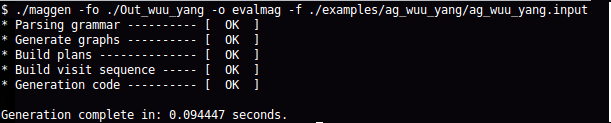
\includegraphics[width=350pt,height=70pt]{normal.png}
\caption{\label{fig:outnormal} Usando \maggen\ con opciones.}
\end{figure}

\item Si invocamos a \maggen\ sin la opción \texttt{-f} (independientemente que usemos o no las demas opciones) se espera la entrada por entrada estándar. Esto nos permite poder utilizar a \maggen\ en conjunto con otros comandos, Ejemplo:\\ \texttt{cat file | maggen -fo ./out/}.\\ Esto muestra a \maggen\ en conjunto con \texttt{cat} usando una tuberia (pipe o |).

\end{itemize}

La salida de \maggen\ esta ordenada a través de directorio bien definidos que marcan el proceso de funcionamiento de la herramienta en casa etapa. A continuación analizaremos la salida de \maggen\ para la invocación:

\texttt{./maggen -fo ./Out\_wuu\_yang -o maggen -f ./examples/ag\_wuu\_yang/ag\_wuu\_yang.input}.


La totalidad de la información generada por la herramienta es mostrada en la figura \ref{fig:outmagegn}. Dicha información es almacenada en la ruta \texttt{./Out\_wuu\_yang}  Podemos observar:
\begin{description}
\item [Archivos maggen.cpp y maggen.cpp] Código C++ del evaluador estático. Es la \textbf{salida principal de} \maggen.
\item [Archivos Plan.hpp y Node.hpp] Código C++ con definiciones y declaraciones necesarias para la ejecución de ``maggen''.
\item [Archivo ``Grammar\_mag.log''] Este contiene la gramática parseada. Se debe tener en cuenta el análisis de este archivo, esto permite encontrar posibles errores en la interpretación del archivo de entrada a \maggen. Tal como se muestra la gramática en este archivo, es la que la herramienta a utilizado para la generación del evaluador.
\item [Directorio ``graphs''] Contiene los 4 tipos de grafos construidos por \maggen\ en el proceso visto en la sección \ref{subsec:graph}. Los mismos están ordenados por 4 directorios diferentes denominados: \textit{1\_DP\_graphs}, \textit{2\_DOWN\_graphs}, \textit{3\_DCG\_graphs}, \textit{4\_ADP\_graphs}. Cada unos de ellos contiene archivos \texttt{.dot} para cada grafo creado. Este directorio, además, es utilizado para el caso que se detecte planes cíclicos, donde se almacenan los grafos que producen dependencias cíclicas en un solo directorio y se omiten los demas grafos.
\item [Directorio ``plans''] Contiene archivos \texttt{.dot} con los planes generados por \maggen.
\item [Directorio ``directorio plans project''] Contiene archivos \texttt{.dot} con los planes proyectados generados por \maggen.
\end{description}

\begin{figure}\centering
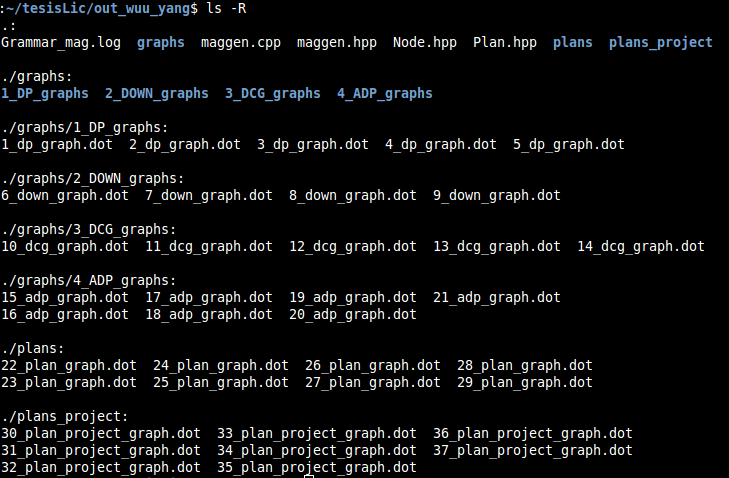
\includegraphics[width=350pt,height=229pt]{out_all.png}
\caption{\label{fig:outmagegn} Salida de \maggen: Directorios y archivos.}
\end{figure}


\section{Uso del evaluador generado}
Para el usos del evaluador generado por \maggen\ necesitamos los 4 archivos generados en el directorio de salida, siguiendo con la salida de la seccion anterior, ellos son:
\begin{itemize}
\item maggen.hpp.
\item maggen.cpp.
\item Plan.hpp.
\item Node.hpp.
\end{itemize}
El evaluador generado por \maggen\ puede ser usado como un modulo C++ en conjunto con otro proyecto. En esta seccion seguiremos con un ejemplo el uso del evaluador para el ejemplo Wuu Yang, el cual se ha tratado en los capitulos anteriores (Ver entrada a \maggen\ en el apendice \ref{append:agwuuyang}).

Como bien hemos visto en secciones anteriores, la entrada del evaluador generado por \maggen\ es un AST. El siguiente módulo de código C++ describe un AST para la gramática del ejemplo de Wuu Yang.

\tiny
\lstinputlisting[numbers=left, numberstyle=\tiny, numbersep=5pt, language=c++]{input_file_code/ast.cpp}
\normalsize

Observemos el AST con el siguiente diagrama:
\begin{center}
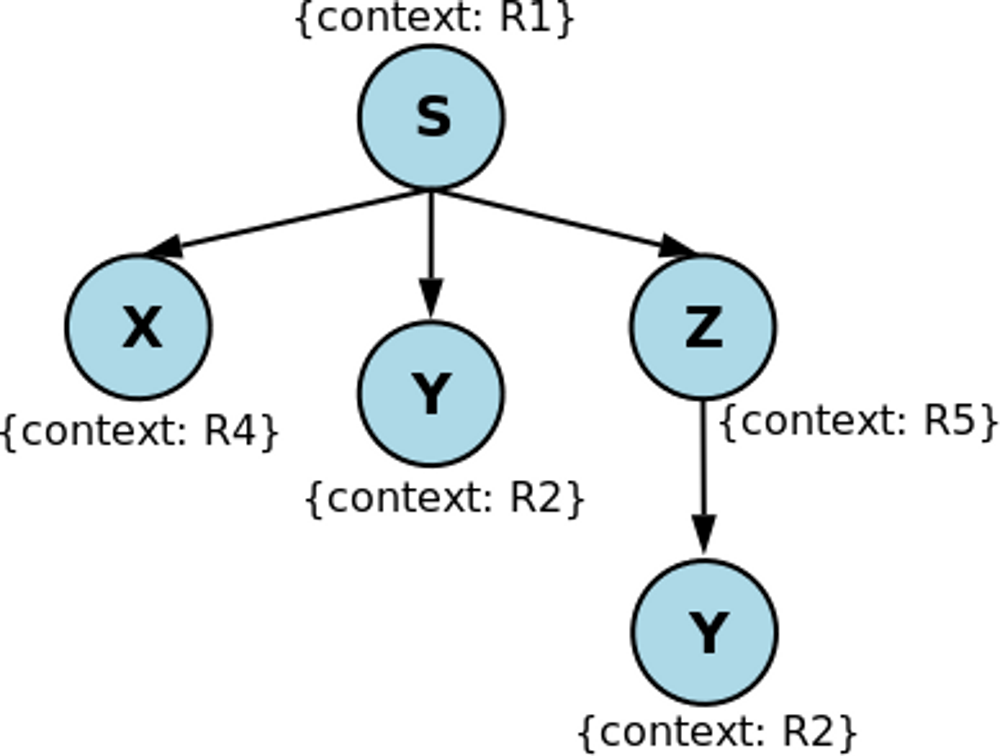
\includegraphics[width=250pt,height=193pt]{ast.png}
\end{center}
Los atributos de cada símbolo del AST esta con valores indefinidos, veamos en la siguiente imagen con la compilación e invocación del evaluador generado por \maggen\ para computar los atributos de los símbolos del AST.
\begin{center}
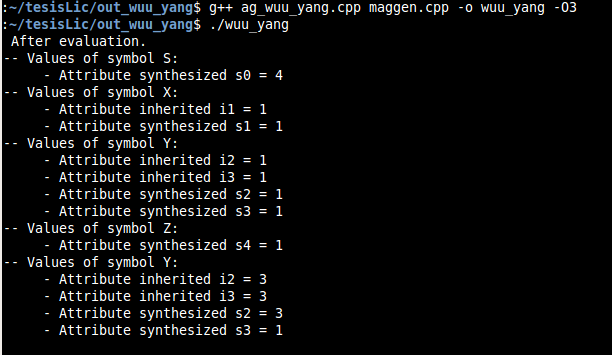
\includegraphics[width=350pt,height=203pt]{ast-computed.png}
\end{center} 

Analicemos los valores de los atributos de cada símbolo en la siguiente tabla:
\begin{center}\begin{tabular}{|| c | c | l ||}
\hline \hline

\rowcolor[rgb]{0.8, 0.8, 0.8} \textbf{Símbolo}&\textbf{Atributo}&\textbf{Evaluación}\\ \hline

\multirow{2}{*}{\textbf{S}} & \multirow{2}{*}{s0} & \texttt{(eq 1) S.s0 = X.s1 + Y.s2 + Y.s3 + Z.s4} \\ 
                           &                     & \textbf{S.s0 = 4} \\ \hline

\multirow{4}{*}{\textbf{X}} & \multirow{2}{*}{i1} & \texttt{(eq 2) X.i1 = Y.s3} \\ 
                           &                     & \textbf{X.i1 = 1.} \\ \cline{2-3}
                           & \multirow{2}{*}{s1} & \texttt{(eq 9) X.s1 = X.i1} \\ 
                           &                     & \textbf{X.s1 = 1.} \\ \hline

\multirow{7}{*}{\textbf{Y}} &                 s3  & \texttt{(eq 6)} \textbf{Y.s3 = 1} \\ \cline{2-3}
                           & \multirow{2}{*}{s2} &    \texttt{(eq 5) Y.s2 = Y.i2} \\
                           &                     & \textbf{Y.s2 = 1} \\ \cline{2-3}
                           & \multirow{2}{*}{i2} & \texttt{(eq 3) Y.i2 = X.s1} \\
                           &                     & \textbf{Y.i2 = 1} \\ \cline{2-3}
                           & \multirow{2}{*}{i3} & \texttt{(eq 4) Y.i3 = Y.s2} \\
                           &                     & \textbf{Y.i3 = 1} \\ \hline

\multirow{2}{*}{\textbf{Z}} & \multirow{2}{*}{S4} & \texttt{(eq 10) Z.s4 = Y.s3} \\
                           &                     & \textbf{Z.s4 = 1} \\ \hline

\multirow{7}{*}{\textbf{Y}} &                  s3 & \texttt{(eq 6)} \textbf{Y.s3 = 1} \\ \cline{2-3}
                           & \multirow{2}{*}{s2} &    \texttt{(eq 5) Y.s2 = Y.i2} \\
                           &                     & \textbf{Y.s2 = 3} \\ \cline{2-3}
                           & \multirow{2}{*}{i2} & \texttt{(eq 3) Y.i2 = X.s1} \\
                           &                     & \textbf{Y.i2 = 3} \\ \cline{2-3}
                           & \multirow{2}{*}{i3} & \texttt{(eq 4) Y.i3 = Y.s2} \\
                           &                     & \textbf{Y.i3 = 3} \\
\hline \hline


\end{tabular}\end{center}

\begin{figure}\centering
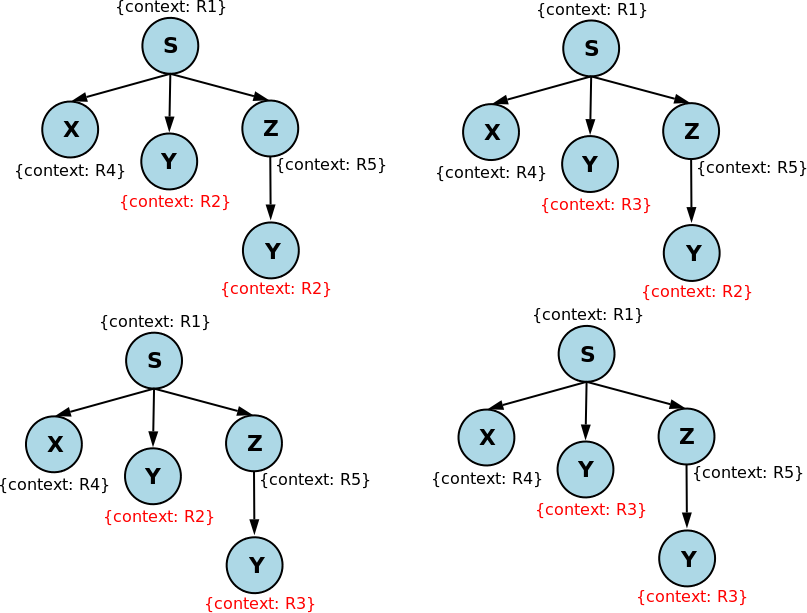
\includegraphics[width=350pt,height=257pt]{ast-all.png}
\caption{\label{fig:allast} AST para ejemplo de Wuu Yang.}
\end{figure}

Tal como analizamos en el ejemplo anterior, el evaluador generado por \maggen\ podría ser utilizado con todos lo AST posibles. Esto es, debido a que el evaluador contiene las secuencias de visita previamente computadas para hacer la tarea de evaluación con una notoria ganancia de tiempo. Entonces podríamos invocar al evaluador, además, con los demas AST que se desprenden con la gramática del ejemplo de Wuu Yang. En la figura \ref{fig:allast} podemos ver la totalidad de AST.

Notar que el ejemplo Wuu yang analizado es considerablemente simple, pero podemos encontrar gramáticas muy simples en la cual los posibles AST sea una cantidad considerable, es en este punto donde el evaluador generado por \maggen\ adquiere mayor potencial y utilidad.

\section{Mensajes y avisos}

En la siguiente tabla analizamos la descripcion de los posibles errores y aviso que se deben tener en cuenta cuando usamos \maggen.
\newpage
\begin{longtable}{| p{5cm} || p{5cm} | p{5cm} |}
\caption{Tabla con mensajes de error en \maggen.}\label{table:mensajes}\\ 
\hline

\rowcolor[rgb]{0.8, 0.8, 0.8} \textbf{Mensaje} & \textbf{Descripcion} & \textbf{Ayuda}\\
\hline

ERROR: operator non-associtive using wrong use \ldots & bla bla & no se.\\ \hline
ERROR: Symbol Non-Teminal \textit{SYMBOL} uses in the right part without rule & bla bla & nose \\ \hline
ERROR: \textit{SYMBOL} [ \textit{NUM} ]. \textit{ATTR} type synthetized, haven't an equation that defines it. & bla bla & nose \\ \hline
ERROR: \textit{SYMBOL} [ \textit{NUM} ].\textit{ATTR} type inherited, haven't an equation that defines it. & bla bla & nose \\ \hline

ERROR: \textit{SYMBOL} [ \textit{NUM} ].\textit{ATTR} type synthetized, is defined outside his scope. & bla bla & nose \\ \hline


ERROR: the file input non-exist & blabla & noose \\ \hline
ERROR: Parsing Failed, the following text will not be able to parse: \ldots & bla bla & nose \\ \hline

ERROR: non-terminal symbol \textit{SYMBOL} used does not belong to the rule: \textit{RULE} & bla bla & nose \\ \hline
ERROR: Index \textit{NUM} of symbol  \textit{SYMBOL} incorrect. & bla bla & nose \\ \hline 
ERROR: \textit{ATTR} Attribute non-existent. Check the attributes used in the symbols. & bla bla & nose. \\ \hline
ERROR: Type not expected from l\_value." & bla bla & nose \\ \hline 
ERROR: infix operator non-exist: \textit{OP-INFIX}. & bla bla & nose \\ \hline 
ERROR: Function non-exist: \textit{FUNCTION}. & bla bla & nose \\ \hline 
ERROR: postfix operator non-exist: \textit{OP-POSFIX}. & bla bla & nose \\ \hline 
ERROR: prefix operator non-exist: \textit{OP-PREFIX}. & bla bla & nose \\ \hline 
ERROR: The grammar isn't extended grammar. & bla bla & nose \\ \hline
ERROR: the path \textit{PATH} is invalid or inaccessible. & bla bla & nose \\ \hline
ERROR: One o more graph ADP has an cycle in its dependencies. Look the folder \textit{PATH-OUTPUT}. & bla bla & nose \\ \hline 
ERROR: Path non exist: \textit{PATH}. & bla bla & nose \\ \hline 
ERROR: maggen wrong uses. & bla bla & nose \\ \hline




ERROR: the AST input is wrong create. & bla bla & nose \\ \hline
ERROR: the AST input is wrong create. & bla bla & nose \\ \hline
ERROR: Fatal action. & bla bla & nose \\ \hline
ERROR: Index out bounds: combined ADP graphs.& bla bla & nose \\ 
\hline 

\end{longtable}
